\section{Introduction}\label{sec:intro}

For a graph $G=(V,E)$ with one variable $z_e$ per edge, the perfect-matching polynomial is
\[
  P_G(z)=\sum_{M\in\PM(G)}\ \prod_{e\in M} z_e .
\]
Valiant~\cite{Valiant80,Valiant79} studied a family of triangular grids $G_r$ with $\Theta(r^2)$ vertices. He proved that every monotone arithmetic circuit for $P_{G_r}$, meaning one with no subtraction, has size at least $c^r$ for a constant $c>1$ \cite[Thm.~1]{Valiant80}. With subtraction, Kasteleyn's Pfaffian method computes $P_{G_r}$ with polynomially many operations \cite[Thm.~2]{Valiant80}. The lower bound relies on a local property of the triangular lattice, his Lemma~8. On the last page he writes:
\begin{quote}
``In conclusion we note that our Lemma 8 is false for regular rectangular grids. The monotone complexity of these closely related polynomials is therefore unresolved.'' \cite[p.~313]{Valiant80}
\end{quote}

This paper treats the free $L\times L$ square grid with $L$ even. We write $P_L$ for its perfect-matching polynomial and $U_L$ for the uniform distribution on its perfect matchings (domino tilings), viewed as a distribution on $\{0,1\}^n$ with $n=2L(L-1)$ edge indicators. Throughout, $0\le\eps\le1$ denotes a total-variation error. We prove the following.
\begin{itemize}
\item Every monotone arithmetic circuit for $P_L$, and every $(\min,+)$ circuit for the minimum-weight perfect matching on the grid, has size at least $\exp(c(L)L)$. Here $c(L)\ge 1/1129$ for $L\ge1000$. A transfer-matrix circuit of size $O(L^2(1+\sqrt2)^L)$ shows that this is tight up to the constant in the exponent (Theorems~D and~C).
\item Every nonnegative, smooth, decomposable probabilistic circuit (PC) with leaves of arity at most $2n/3$ whose distribution is within total variation $\eps<1$ of $U_L$ has size at least $(1-\eps)^2\exp(c(L)L)$. Determinism is not assumed (Theorem~B). So the optimal size of such circuits is $\exp(\Theta(L))=\exp(\Theta(\sqrt n))$, both for exact representation and for every fixed error below one.
\end{itemize}
Both lower bounds rest on one probability estimate, Theorem~A and its vertex-cut variant Theorem~A$'$. For every split $E=A\sqcup B$ of the edges with $\abs A,\abs B\ge n/3$ and every vertex set $S$,
\[
  U_L\bigl(\text{the edges of } M \text{ in } A \text{ cover exactly } S\bigr)\ \le\ e^{-c(L)L}.
\]
For the Rokhsar--Kivelson state on the square this says that the R\'enyi-$\infty$ entropy is at least $c(L)L$ across every balanced bipartition of the links (Corollary~\ref{cor:entanglement}).

We have not found a later resolution of the square case in the literature. Our search (Section~\ref{sec:related}) was targeted, not exhaustive.

\subsection{What already follows from Valiant's argument}\label{sec:intro-triangular}

A robust separation of the same kind already follows from Valiant's proof, so we state it first. The intermediate counting statement in his proof of Theorem~1 \cite[pp.~311--312]{Valiant80} is stronger than the theorem. For every vertex partition of $G_r$ into two parts of comparable size, the fraction of perfect matchings with no edge across the partition is $\exp(-\Omega(r))$. Section~\ref{sec:vertex-route} shows that such a counting statement, combined with standard degree homogenization and an overlap bound, gives a constant-TV lower bound for nonnegative decomposable PCs with univariate leaves.

\begin{proposition}[Valiant's argument, robust form]\label{prop:triangular}
Let $G_r$ be Valiant's triangular grid, with $r(r+1)/2$ vertices, for those $r$ where it has perfect matchings. Let $T_r$ be the uniform distribution on its perfect matchings, as a distribution on edge indicators. There are constants $c_0>0$ and $r_0$ such that for $r\ge r_0$:
\begin{enumerate}[label=(\alph*)]
\item every nonnegative smooth decomposable PC with univariate leaves whose distribution $Q$ satisfies $\TV(T_r,Q)\le\eps$ has size at least $(1-\eps)^2e^{c_0r}/\mathrm{poly}(r)$;
\item the generating polynomial $\sum_x T_r(x)z^x$ has an arithmetic circuit of size $\mathrm{poly}(r)$ that uses subtraction, that is, a polynomial-size probabilistic generating circuit in the sense of~\cite{ZhangJubaVdB21}.
\end{enumerate}
For every fixed error below one, part (a) gives size $\exp(\Omega(r))$.
\end{proposition}

Part (b) is Valiant's Theorem~2 after normalization: Kasteleyn's Pfaffian gives every matching the same sign. Part (a) combines Valiant's Lemmas~6--8 and Corollary~9, as used in his proof of Theorem~1, with two standard steps. The proof is in Section~\ref{sec:vertex-route}. We have not found (a) stated in this form. It is still best read as a corollary of 1980 techniques. In particular, the existence of an exponential constant-TV gap between nonnegative decomposable PCs and determinant-based circuits on a natural planar lattice is not new. Generic separations of this type with $\exp(\Omega(n))$ size also follow from older code constructions (Section~\ref{sec:codes}). The contribution of this paper is the square-grid package: Theorems~A, A$'$, B, C and D, and the analytic proof behind them.

\subsection{What fails on the square lattice}\label{sec:intro-fails}

Valiant's proof has three combinatorial ingredients.
\begin{itemize}
\item \textbf{Lemma 6}: a balanced vertex partition of $G_r$ is crossed by $\Omega(r)$ edges. Valiant notes that an analogue for square grids appears in~\cite{DeMilloEisenstatLipton75}.
\item \textbf{Lemma 7}: one can choose $\Omega(r)$ crossing edges that are far from each other and from the sides. Our Lemma~\ref{lem:select-vertex} is a square-grid version.
\item \textbf{Lemma 8 and Corollary 9}: local replaceability. Lemma~8 concerns $G_r$ with $r=12i+10$ and a \emph{radius} $e$, an edge at the centre. It says that every \emph{remnant} of $G_r$ (the grid minus some vertices on its sides) that has a perfect matching has one containing $e$. For the fixed patch $G_{22}$, Corollary~9 turns this into a uniform ratio $K>1$ between all perfect matchings of a remnant and those avoiding $e$. The proof of Theorem~1 multiplies these ratios over $\Omega(r)$ disjoint patches.
\end{itemize}
The third ingredient has no square-lattice analogue for any patch size.

\begin{proposition}[the square analogue of Lemma 8 fails]\label{prop:flux}
Let $m\ge2$ be even. Let $W_m=\{1,\dots,m\}^2\subset\Z^2$ and let $e$ be one of the four edges joining two of the four central vertices of $W_m$. Then there is a set $D$ of vertices on the boundary of $W_m$ such that $W_m\setminus D$ has a perfect matching, but no perfect matching of $W_m\setminus D$ contains $e$.
\end{proposition}

\begin{proof}
Colour $(x_1,x_2)$ black if $x_1+x_2$ is even and white otherwise. A rotation by $90^\circ$ maps horizontal central edges to vertical ones. The reflection $x_1\mapsto m+1-x_1$ swaps the colours, because $m+1$ is odd. So we may assume $e$ is vertical, joins rows $m/2$ and $m/2+1$, and has a white upper endpoint. Let $D$ be the set of white vertices in the top row together with the black vertices in the bottom row.

\emph{A perfect matching exists.} In an odd column $x_1$ the bottom vertex is black and the top vertex is white (since $m$ is even), so both are removed. The remaining rows $2,\dots,m-1$ are paired by vertical dominoes. In an even column nothing is removed, and rows $1,\dots,m$ are paired by vertical dominoes.

\emph{No perfect matching contains $e$.} Let $T$ be the set of remaining vertices in rows $m/2+1,\dots,m$. Each full row has $m/2$ vertices of each colour, and the top row lost its $m/2$ white vertices. So $T$ has $m/2$ more black than white vertices. In a perfect matching, an edge inside $T$ covers one vertex of each colour, and every other vertex of $T$ is matched by a vertical edge crossing the middle line. Hence
\[
  \#\{\text{crossing edges with black top}\}-\#\{\text{crossing edges with white top}\}=m/2 .
\]
Exactly $m/2$ vertical edges cross the middle line with a black upper endpoint. So every perfect matching uses all of them and none with a white upper endpoint. In particular it does not use $e$.
\end{proof}

\begin{figure}[t]
\centering
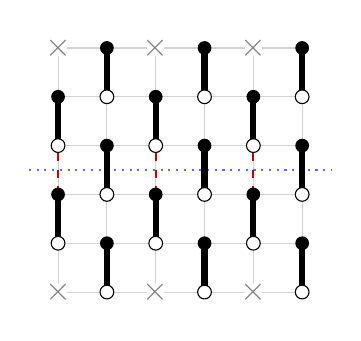
\begin{tikzpicture}[scale=0.62]
  \draw[gray!35] (1,1) grid (6,6);
  \draw[blue!60, dotted, thick] (0.4,3.5) -- (6.6,3.5);
  \foreach \x in {2,4,6} \foreach \y in {1,3,5} \draw[line width=2.2pt] (\x,\y) -- (\x,\y+1);
  \foreach \x in {1,3,5} \foreach \y in {2,4} \draw[line width=2.2pt] (\x,\y) -- (\x,\y+1);
  \foreach \x in {1,3,5} \draw[red!75!black, dashed, thick] (\x,3) -- (\x,4);
  \foreach \x in {1,...,6}{
    \foreach \y in {1,...,6}{
      \pgfmathtruncatemacro{\parity}{mod(\x+\y,2)}
      \ifnum\parity=0 \fill (\x,\y) circle (4pt); \else \draw[fill=white] (\x,\y) circle (4pt); \fi
    }
  }
  \foreach \x in {1,3,5}{
    \fill[white] (\x,6) circle (5pt); \node[gray] at (\x,6) {\large$\times$};
    \fill[white] (\x,1) circle (5pt); \node[gray] at (\x,1) {\large$\times$};
  }
\end{tikzpicture}
\caption{Proposition~\ref{prop:flux} for $m=6$. Crosses mark the removed boundary vertices: white vertices of the top row and black vertices of the bottom row. Thick edges form a perfect matching of the remnant. The dotted line is the middle line. The dashed edges cross it with a white upper endpoint, and no perfect matching of the remnant uses them. A computer check for all even $m\le 30$ is in \texttt{checks/lemma8\_flux.py}.}
\label{fig:flux}
\end{figure}

Boundary conditions can freeze square-lattice edges at distance $m/2$ from the patch boundary. This is the height-function rigidity of square-lattice dimers. Valiant's step of multiplying local ratios is therefore unavailable. We replace it with a global estimate. Fix a set $F$ of $t$ forbidden edges, one in each of $t$ rows spaced three apart. A tilted Kasteleyn determinant gives the identity $\E[(1-\eta)^{\abs{M\cap F}}]=\det(I-\eta H)$, where $H$ is a $t\times t$ matrix of inverse-Kasteleyn entries (Lemma~\ref{lem:tilted}). Carleman's inequality bounds this determinant using only $\tr H$, which is about $t/4$ because bulk edge marginals are near $1/4$, and $\norm{H}_F^2$. The entries of $H$ decay like $1/\abs{i-j}$, and $\sum_k k^{-2}$ converges, so $\norm{H}_F^2=O(t)$. This gives $\Pr(M\cap F=\emptyset)\le e^{-\Omega(t)}$ with no independence assumption and no local replaceability.

\subsection{Results}\label{sec:intro-results}

Section~\ref{sec:results} states the formal versions:
\begin{itemize}
\item \textbf{Theorem A} (edge profiles). For every even $L\ge264$, every split $E=A\sqcup B$ with $\abs A,\abs B\ge n/3$, and every $S\subseteq V$, the profile event $\{\prof_A(M)=S\}$ has probability at most $e^{-c(L)L}$. The function $c(L)$ is explicit and nondecreasing, with $c(400)\ge1/7980$, $c(1000)\ge1/1129$ and $c(L)\to1/(357.2361493\ldots)$
\item \textbf{Theorem A$'$} (vertex cuts). The same bound holds for the event that no edge of $M$ joins $S$ to $V\setminus S$, for every $S$ with $L^2/3\le\abs S\le 2L^2/3$.
\item \textbf{Corollary~\ref{cor:entanglement}} (min-entropy). Across every link bipartition with at least $n/3$ links on each side, the Rokhsar--Kivelson state on the free square has R\'enyi-$\infty$ entanglement entropy at least $c(L)L$.
\item \textbf{Theorem B} (robust PC lower bound). Nonnegative smooth decomposable PCs with leaves of arity at most $2n/3$ that are $\eps$-close to $U_L$ in TV have size at least $(1-\eps)^2e^{c(L)L}$.
\item \textbf{Theorem C} (upper bound). A smooth, decomposable, deterministic PC with indicator leaves computes $Z_L\cdot U_L$ exactly with size at most $3L^2(1+\sqrt2)^L+2n$. A binary, structured version has size at most $6L^2(1+\sqrt2)^L+2n$.
\item \textbf{Theorem D} (exact monotone and tropical). Every monotone arithmetic circuit for a polynomial whose monomials are exactly the perfect matchings of the grid, with any positive coefficients, has size at least $e^{c(L)L}$. Every $(\min,+)$ circuit for the minimum-weight perfect matching on nonnegative weights has the same bound. The proof goes through Theorem~A$'$, which plays the role of Valiant's Corollary~9.
\item \textbf{Signed circuits} (Section~\ref{sec:signed}). The Kasteleyn determinant gives a polynomial-size generating circuit for $U_L$ that uses subtraction. Known conversions \cite{AgarwalBlaser24,BroadrickZhangVdB24} turn it into a polynomial-size signed circuit for the network polynomial, but that circuit is not syntactically decomposable. For signed \emph{structured}-decomposable circuits with univariate leaves, exact representation needs size at least $e^{c(L)L}-1$ (Proposition~\ref{prop:structured-signed}). For signed unstructured decomposable circuits with univariate leaves the question is open.
\end{itemize}

\begin{table}[t]
\centering
\small
\begin{tabular}{@{}p{5.6cm}p{2.7cm}p{2.9cm}p{2.4cm}@{}}
\toprule
Model (target $P_L$, $\OPT_L$ or $U_L$) & lower bound & upper bound & where\\
\midrule
monotone arithmetic circuit for $P_L$ & $e^{c(L)L}$ & $O(L^2(1+\sqrt2)^L)$ & Thm D, C\\
$(\min,+)$ circuit for $\OPT_L$, weights $\ge0$ & $e^{c(L)L}$ & $O(L^2(1+\sqrt2)^L)$ & Thm D, C\\
nonnegative smooth decomposable PC, leaf arity $\le2n/3$, TV $\le\eps$ & $(1-\eps)^2e^{c(L)L}$ & $O(L^2(1+\sqrt2)^L)$ & Thm B, C\\
signed structured-decomposable, univariate leaves, exact & $e^{c(L)L}-1$ & $O(L^2(1+\sqrt2)^L)$ & Prop \ref{prop:structured-signed}, Thm C\\
signed decomposable (unstructured), univariate leaves & \textbf{open} & $O(L^2(1+\sqrt2)^L)$ & Sec.~\ref{sec:signed}\\
signed circuit for the generating polynomial (PGC) & --- & $\mathrm{poly}(n)$ & Sec.~\ref{sec:signed}\\
\bottomrule
\end{tabular}
\caption{Sizes for the square-grid targets. Here $n=2L(L-1)$, $L$ is even, and $c(L)\ge1/1129$ for $L\ge1000$. For every fixed error below one, the nonnegative PC row gives size $\exp(\Theta(L))$. The upper bound $\ln(1+\sqrt2)\approx0.881$ in the exponent and the certified lower bound $c(L)$ differ by a factor of about $10^3$.}
\label{tab:summary}
\end{table}

\subsection{What this paper does not claim}\label{sec:intro-scope}

\begin{itemize}
\item \textbf{No general separation is claimed.} Proposition~\ref{prop:triangular} and the code example of Section~\ref{sec:codes} already give constant-TV separations between nonnegative decomposable PCs and models with efficient exact inference. The code example even gives $\exp(\Omega(n))$. Our results concern the square grid.
\item \textbf{This is a representation-size result.} For $U_L$, evidence probabilities, marginals, conditionals and exact samples are all computable in polynomial time with planar Kasteleyn determinants (Section~\ref{sec:signed}).
\item \textbf{The constants are crude.} The certified rate $1/1129$ at $L=1000$ is about 100 times smaller than the observed decay rate along the same forbidden sets (Section~\ref{sec:constants}). The bounds say nothing explicit for $L<264$.
\item \textbf{Scope.} We cover the free square with even $L$ and edge-indicator variables. We do not cover rectangles, the torus, or other encodings such as vertex-partner variables (Section~\ref{sec:open}).
\end{itemize}

\subsection{Organization}
Section~\ref{sec:prelim} fixes notation and circuit models. Section~\ref{sec:results} states Theorems~A and~A$'$ and the entanglement corollary. Sections~\ref{sec:kasteleyn}--\ref{sec:selection} prove them: Kasteleyn algebra and Carleman's inequality, the free-square kernel bound, and the selection lemmas with explicit constants. Section~\ref{sec:circuits} derives the circuit lower bounds (Theorems~B and~D and Proposition~\ref{prop:triangular}). Section~\ref{sec:upper} gives the matching upper bound. Section~\ref{sec:signed} discusses signed weights. Sections~\ref{sec:related} and~\ref{sec:open} cover related work and open problems. Appendix~\ref{app:checks} lists the numerical checks.
